\chapter[Background Study]{Chapter 2: Background Study}\label{chap:BG_Study} %Two to three pages long.
%*****************************************************************************************************%
\section{Trending Literature}\label{sec:media1} %BMS Lit of popular media.
%*****************************************************************************************************%
The landscape of battery technology has been rapidly evolving to meet the escalating demands for energy storage solutions, primarily driven by the global transition towards electric vehicles (EVs) and renewable energy. The heart of this evolution lies in the Battery Management Systems (BMS) that ensure safe and efficient operation of batteries, forming a critical component of high voltage battery banks in EVs and grid storage.\newline\newline
\noindent
Recent trends spotlight the shift towards designing scalable modular systems in BMS to accommodate the high voltage requirements. The modular BMS segment, for instance, is projected to register the highest growth rate owing to its ability to connect in series or parallel circuits, thereby augmenting the power/voltage output with the fringe benefit of lower maintenance costs\cite{GlobeNewswire2023}. This indicates a move towards developing flexible and scalable BMS architectures that can seamlessly adapt to varying voltage requirements, essential for high voltage battery banks.\newline\newline
\noindent
In the quest for more affordable and safer electric vehicles, continuous innovation in BMS architectures is pivotal. It's not just about managing existing battery chemistries, but also about being prepared for new and emerging ones. Solid-state batteries, for example, promise more energy in a smaller space, faster charging times, and enhanced safety, which BMS designs need to accommodate\cite{MITTechReview2023}.\newline
\begin{figure}[h!]
\centering
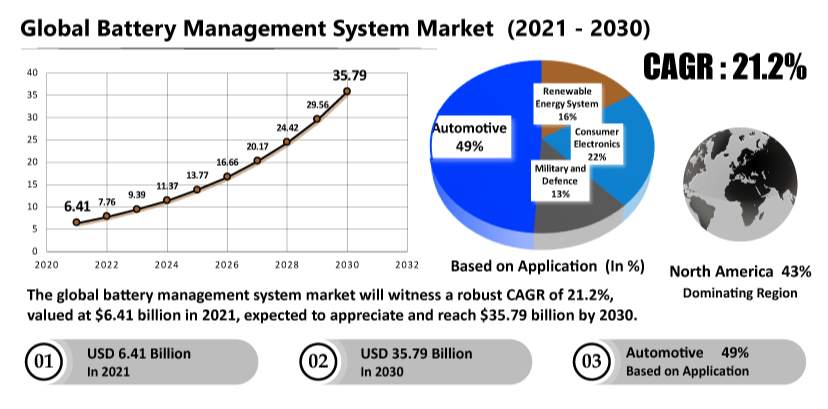
\includegraphics[width=1.0\textwidth]{Skripsie_LaTeXTemplate/Figures/forecast.png}
\caption{Projected Forecast of the BMS Market \cite{m_and_m}}
\label{fig:grow_some}
\end{figure}
\newpage
\noindent
The market's trajectory further corroborates the booming interest in BMS technologies. The global BMS market size, which stood at USD 7.8 billion in 2022, is on a steep ascent, poised to touch USD 55.1 billion, driven by the quest for reducing the cost of battery electronics and simplifying designs to cut down on hardware and wiring costs\cite{BMSSummit2023}.\newline\newline
\noindent
Moreover, the technological advancements by companies like Vitesco Technologies underscore the industry's momentum. With orders worth over 2 billion euros for its innovative BMS, the future seems propitious for further ingenuity in BMS designs, underlining the importance of BMS in the broader narrative of renewable energy solutions\cite{BatteriesNews2023}. This burgeoning sector has caught the attention of various stakeholders, invigorating a flurry of activities around BMS technologies, whether it's about reducing costs, enhancing safety, or accommodating new battery chemistries. As this trend continues, the evolution of BMS is deemed to play a cardinal role in propelling the broader adoption of electric vehicles and renewable energy systems, making it a focal point of interest among industry players, researchers, and policymakers.
%*****************************************************************************************************%
\section{High Voltage DC systems}\label{sec:DC_SYST}
%*****************************************************************************************************%
High voltage DC battery storage systems operate at voltages exceeding 96V, with potential levels up to 384V or even 800V \cite{source1}. With cell modules or individual cells in series, the system achieves the desired operational voltage, each unit incrementing the total voltage. The advantage of high voltage configurations lies in the reduction of $I^{2}\cdot R$ losses, as a higher voltage level lowers the current required for a specific power output, enhancing system efficiency. High voltage systems simplify design by reducing parallel strings and current ratings, lowering component costs and easing battery management, which may enhance reliability and lifespan. To comprehend the simplification for a design, I evaluated examples of HV systems and saw that in principal a design can be formulated using straightforward calculations with equations \ref{eq:HV1}, \ref{eq:HV2} \& \ref{eq:HV3}, adjusting the variables below.\newline

\begin{table}[h]
\centering
\caption{Example Parameters for a HV Battery Bank Design\cite{source2}}
\label{tab:parameters}
\begin{tabular}{|p{7cm}|p{4cm}|p{4cm}|}
\hline
\textbf{Parameter} & \textbf{Symbol} & \textbf{Typical Value} \\ \hline
Nominal voltage of cell/module & \( V_{\text{nom}} \) & 48V \\ \hline
Number of cells/modules in series & \( n \) & Variable \\ \hline
Total System Voltage & \( V_{\text{total}} \) & \( n \cdot V_{\text{nom}} \) \\ \hline
Nominal Capacity & \( C_{\text{nom}} \) & 50Ah \\ \hline
Maximum Charging Current & \( I_{\text{charge}} \) & 50A \\ \hline
Maximum Discharging Current & \( I_{\text{discharge}} \) & 50A \\ \hline
Charge Cut-off Voltage & \( V_{\text{charge,cutoff}} \) & 438V \\ \hline
Discharge Cut-off Voltage & \( V_{\text{discharge,cutoff}} \) & 300V \\ \hline
\end{tabular}
\end{table}
\newpage
\begin{equation}
V_{\text{total}} = n \cdot V_{\text{nom}}
\label{eq:HV1}
\end{equation}
\begin{equation}
C_{\text{total}} = C_{\text{nom}}
\label{eq:HV2}
\end{equation}
\begin{equation}
E_{\text{total}} = V_{\text{total}} \cdot C_{\text{total}}
\label{eq:HV3}
\end{equation}\newline
\noindent
These equations form the basis for designing high voltage battery banks. The modularity of the design allows for scalability; additional modules can be connected in series to increase the voltage or in parallel to increase the capacity, thereby accommodating varying energy storage needs. The operational parameters like maximum charging and discharging currents are crucial to ensure the safety and efficiency of the system.\cite{source3}\newline\newline
\noindent
In summary, the theoretical formulation of a high voltage battery bank hinges on the series connection of cells/modules, with the total system voltage and capacity governed by the nominal voltage and capacity of individual cells/modules. This modular and scalable design is fundamental to meeting the diverse energy storage requirements across different applications.
%*****************************************************************************************************%
\section{Lithium Ferro Phosphate Technology}\label{sec:LFP}
%*****************************************************************************************************%
\textbf{\emph{Chemistry of LFP Cells}}\newline
\noindent
Lithium Iron Phosphate (LiFePO4 or LFP) cells function through the process of lithium ions moving from the cathode to the anode and vice versa during discharge and charge cycles, respectively. This movement, termed intercalation (insertion) during discharge and deintercalation (extraction) during charge, facilitates the storage and release of electrical energy. The primary components of an LFP cell are its cathode, composed of lithium iron phosphate, its anode made of graphite, and the electrolyte, a lithium salt dissolved in an organic solvent. The cathode serves as the source and sink of lithium ions, enabling the reversible electrochemical reactions crucial for the cell's energy storage and delivery.\cite{LiFePO4Wiki}\newline\newline
\noindent
$Discharge$
\[ \text{Cathode: } \text{LiFePO}_4 \rightarrow \text{FePO}_4 + \text{Li}^+ + e^- \]
\[ \text{Anode: } \text{LiC}_6 + \text{Li}^+ + e^- \rightarrow 6\text{C} \]
$Charge$
\[ \text{Cathode: } \text{FePO}_4 + \text{Li}^+ + e^- \rightarrow \text{LiFePO}_4 \]
\[ \text{Anode: } 6\text{C} \rightarrow \text{LiC}_6 \]
\newpage
\noindent
\textbf{\emph{Typical Data Specs}}\newline
\noindent
- \emph{Nominal Voltage}: $3.2V$\newline
- \emph{Energy Density}: $90 Wh/kg$ - $120 Wh/kg$\newline
- \emph{Cycle Life}: $>2000$ cycles ($80\%$ DoD)\newline
- \emph{Charge/Discharge Efficiency}: $95\%$ - $98\%$\newline
- \emph{Operating Temperature Range}: $-20^{o}C$ to $60^{o}C$\newline\newline
\noindent
\textbf{\emph{C Rating}}\newline
\noindent
The C rate denotes the rate at which a battery is charged or discharged, calculated as:
\[ \text{C Rate} = \frac{\text{Current (A)}}{\text{Capacity (Ah)}} \]
\noindent
\textbf{\emph{Discharge Current}}\newline
\noindent
For a 100Ah cell with a 1C rate, the current capability for 1 hour of constant discharge is:
\[ \text{Current (A)} = \text{C Rate} \times \text{Capacity (Ah)} = 100A \]
\noindent
\textbf{\emph{Charge Current}}\newline
\noindent
Selection of charge current, guided by manufacturer specifications, affects charging time, heat generation, and cell lifespan.\newline\newline
\noindent
\textbf{\emph{Cells in Series}}\newline
\noindent
In series connections, voltage accumulates while capacity remains constant, necessitating careful management to prevent overcharge or over-discharge.\newline\newline
\noindent
\textbf{\emph{Cell Balancing}}\newline
\noindent
Balancing ensures equal state of charge (SoC) in series-connected cells, employing active or passive techniques to prevent overcharge or over-discharge.\newline\newline
\noindent
\textbf{\emph{Cell Comparison}}
\begin{table}[h]
    \centering
    \caption{Cell Types \cite{cell_COMP1}\cite{cell_COMP2}}
    \label{tab:cell_comparison}
    \begin{tabular}{|p{2.7cm}|p{3.8cm}|p{3.8cm}|p{3.8cm}|}
        \hline
        Aspect & LFP (LiFePO4) & NMC (LiNiMnCoO2) & LCO (LiCoO2) \\
        \hline
        Energy Density & $\sim$90-120 Wh/kg & $\sim$150-220 Wh/kg & $\sim$200 Wh/kg \\
        \hline
        Safety & Higher & Lower & Lower \\
        \hline
        Lifespan & $>$2000 cycles & $\sim$1000-2000 cycles & $\sim$500-1000 cycles \\
        \hline
        Cost & Less Expensive & More Expensive & Expensive \\
        \hline
        Thermal Range & -20°C to 60°C (-4°F to 140°F) & -20°C to 55°C (-4°F to 131°F) & -40°C to 70°C (-40°F to 158°F) \\
        \hline
        Industry Usage & $31\%$ & N/A & N/A \\
        \hline
    \end{tabular}
\end{table}

\newpage
%*******************************************%
\section{Battery Cell Monitor and Control}\label{sec:Cell_M}
%*******************************************%
\subsubsection{Battery Management}\label{subsec:BM}
Battery management is pivotal to the evolution and efficiency of battery-operated systems, marking a significant stride from the invention of the first true battery by Alessandro Volta in 1799, to the modern rechargeable batteries pioneered by Gaston Plante in 1859\cite{1}. The burgeoning rise of electric vehicles (EVs) and the global shift towards carbon neutrality underscored the imperative for adept battery performance monitoring and management for enhanced efficiency, safety, and user satisfaction\cite{2}.\newline\newline
\noindent
Historically, the nascent forms of battery management were rudimentary, primarily encompassing basic protection circuits for discharge current tripping, which were unstable. The evolution of electronic protection circuits, integrated into comprehensive battery management systems (BMS), marked a significant advancement, catering to a myriad of battery chemistries\cite{3}. Passive cell balancing emerged as a technique to equalize the State of Charge (SoC) among cells in a battery stack, particularly focusing on cells with lower capacity to ensure balanced performance\cite{4}.\newline\newline
\noindent
With the proliferation of onboard batteries across various applications, the exigency for advanced management burgeoned, precipitating the development of centralized and distributed battery management systems aimed at bolstering battery performance and user experiences\cite{5}. The evolution of batteries was inextricably tied to the products and systems that employed them. The burgeoning demand for improved portable power sources, propelled by the ubiquity of mobile computing and communication, spearheaded innovations in battery management technology\cite{6}.
\subsubsection{Controller Topology}\label{subsec:CnTp}
The controller topologies in Battery Management Systems (BMS) are quintessential for efficient monitoring and regulation of battery packs. These topologies are crafted to meet specific requirements and applications, thereby ensuring the safety and reliability of battery operations.\newline\newline
\noindent
\emph{Centralized Topology:}\newline
\noindent
In a centralized topology, a singular control unit is interfaced with each cell in the battery pack through separate wiring. This control unit is pivotal for monitoring and managing the battery cell parameters, thereby ensuring the safe and reliable operation of the overall battery pack\cite{7}.\newline\newline
\noindent
\emph{Modular Topology:}\newline
\noindent
The modular topology encompasses a master controller, multiple slave controllers, and an electric meter. The master controller orchestrates communication with the slave controllers, each accountable for a subset of battery cells, while the electric meter furnishes pack-level readings. This topology is employed to manage larger battery packs efficiently, offering a scalable solution for battery management\cite{8}.\newline\newline
\noindent
\emph{Distributed Topology:}\newline
\noindent
In a distributed topology, dedicated control units are allocated at a central control unit, each tethered to individual battery cells. This setup facilitates granular control and monitoring of each cell, ensuring swift identification and rectification of any discrepancies in cell performance. Although the control units are dedicated, they are centrally located, not positioned atop each cell, which augments the monitoring efficacy while maintaining a structured control hierarchy\cite{9}.\newline\newline
\noindent
The choice of topology is contingent on the application, size, and configuration of the battery pack, and the requisite level of control and monitoring. The broad spectrum of applications with different voltage classes, necessitates divergent controller topologies to align with the hardware requirements of BMS for a given application. Understanding these topologies and their ramifications on the BMS performance is instrumental for engineers to design and implement efficacious and reliable BMS controllers.
%*******************************************%
\section{Module Communication Methodology}\label{sec:commsMeth}
%*******************************************%
Communication is crucial for the effective functionality of the envisioned system, as it facilitates the transfer of data and enables interaction between individual cells through their respective monitoring modules. A comprehensive investigation was undertaken to discern a communication methodology that aligns seamlessly with the project's overarching objectives. Initial evaluations delved into the Canbus design orchestrated by Stuart Pittaway\cite{stuart_pittaway} and the isoSPI design conceived by Mark Wolf\cite{mark_wolf}, yet both methodologies were deemed incompatible with the project's requirements. Subsequently, the isolated UART serial communication design emerged as a suitable solution, rendering compatibility with the smaller microcontrollers envisaged for the project, and permitting isolation between differing voltage levels across the communication pathway, ensuring a robust communication framework\cite{TIDA00163}.\newline\newline
\noindent
Two principal communication configurations were meticulously explored: the daisy-chain and all-call UART connection configurations, as illustrated in Figures \ref{fig:daisy} and \ref{fig:allcall}, respectively. The daisy-chain configuration links devices in a series, each connected to the next device's RX and TX pins, forming a closed loop, as further elucidated by a reference design from Texas Instruments specifically tailored for battery management applications\cite{TI_UART_SPI_bridgee}. On the other hand, the all-call configuration establishes a parallel connection of devices to a single communication line, with all devices interfacing directly with the master controller's RX and TX pins, thereby centralizing the communication system.

\begin{figure}[!htb]
\centering
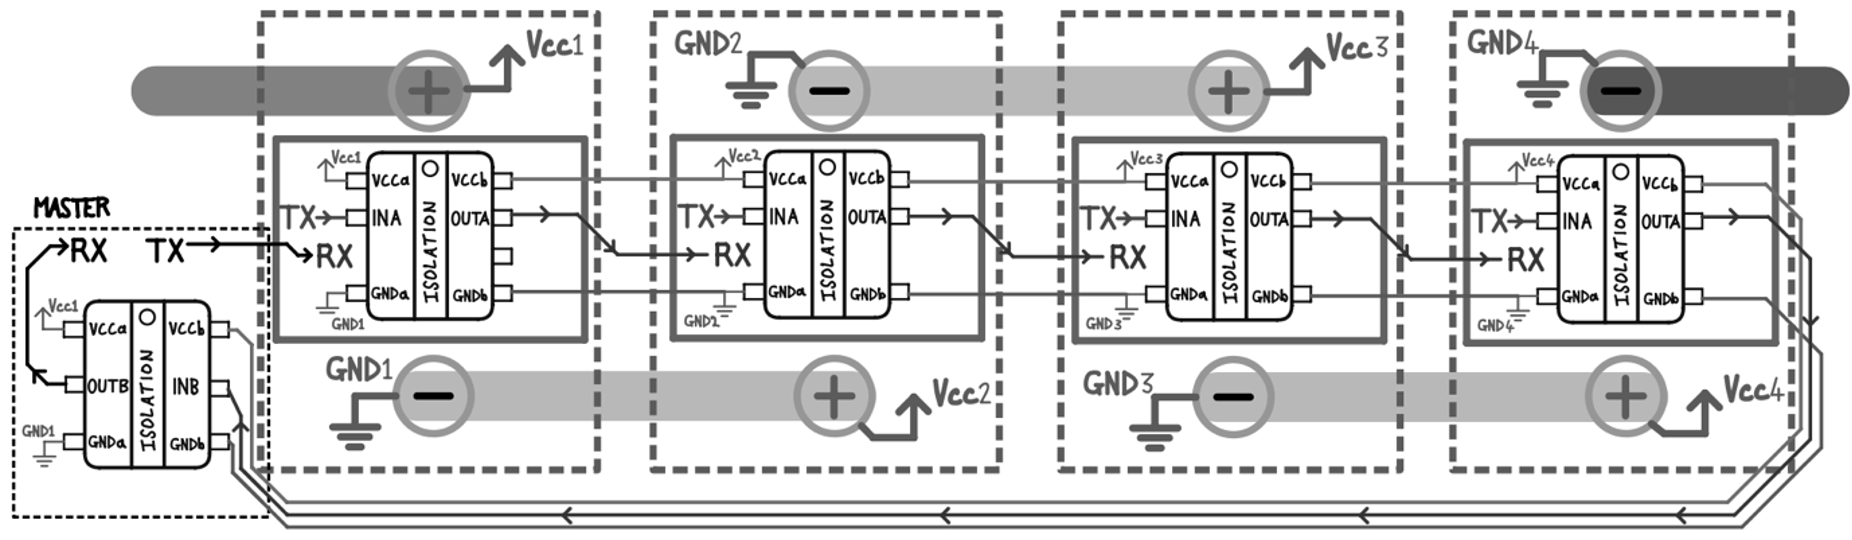
\includegraphics[width=1.0\linewidth]{Figures/DaisyChain.png}
\caption{Daisy-chain configuration.}
\label{fig:daisy}
\end{figure}
\noindent
The depicted diagram above illustrates a daisy-chain architecture among a stack of microcontrollers, where each device transmits messages sequentially, initiating a new cycle upon completion of the loop. Each device in the chain transmits only after successful reception. This allows the modules to receive messages from the other modules within one full cycle.

\begin{figure}[!htb]
\centering
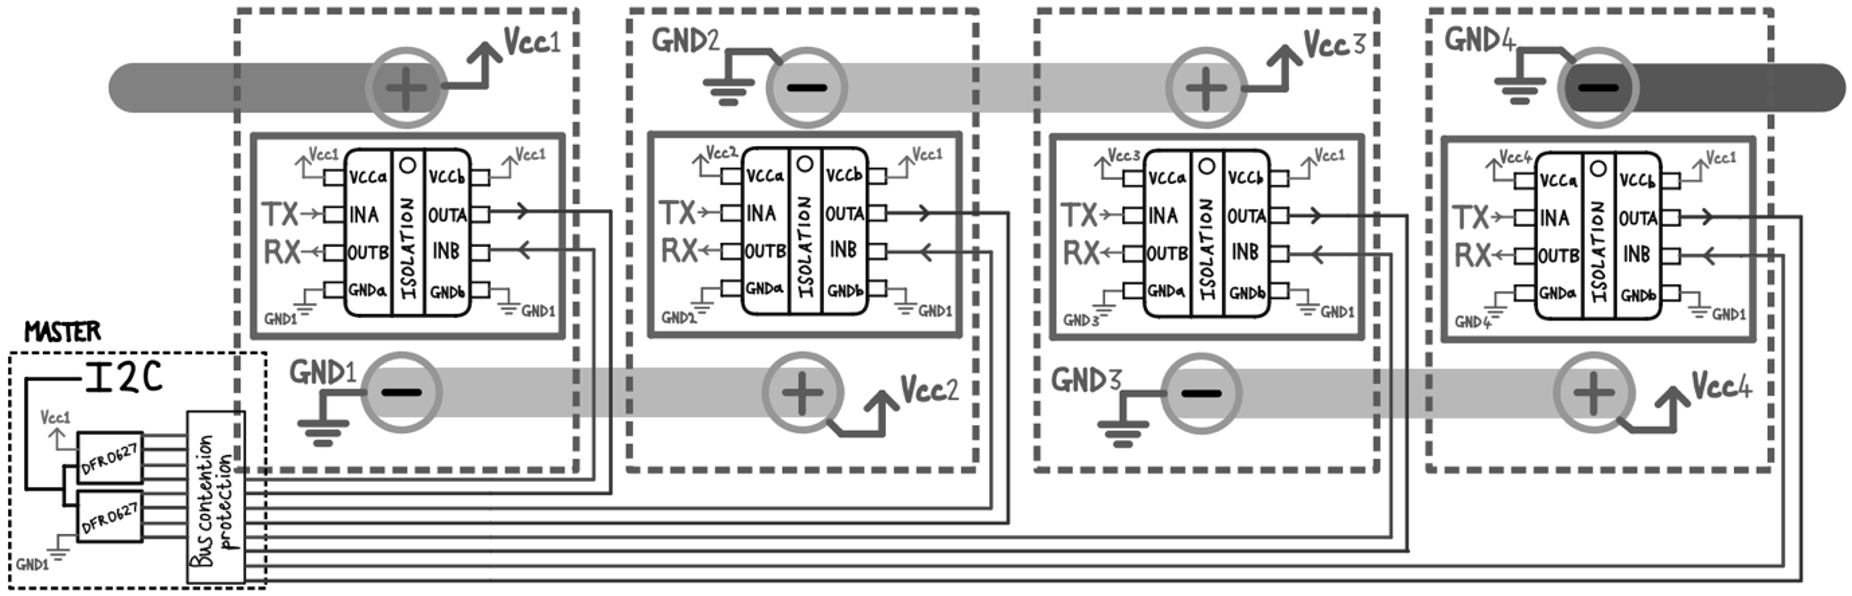
\includegraphics[width=1.0\linewidth]{Figures/AllCall.png}
\caption{All-call configuration.}
\label{fig:allcall}
\end{figure}
\noindent
In the all-call configuration, modules communicate exclusively with the main controller, which operates in parallel with the slave modules. System data exchange among all modules now necessitates two cycles, albeit expedited due to the main controller's broadcast capability.\newline\newline
\noindent
A comparative analysis of these configurations is presented in Table \ref{tab:UART_comparison}, delineating various aspects like hardware and wiring complexity, transmission delay, data rate, software complexity, and fault tolerance.
\newpage
\begin{table}[h]
\centering
\caption{UART Hardware Configuration Comparison}
\label{tab:UART_comparison}
\begin{tabular}{|p{2.2cm}|p{6.1cm}|p{7cm}|}
\hline
\textbf{Feature} & \textbf{Daisy-Chain Configuration} & \textbf{Bus Configuration} \\
\hline
Definition & Devices are connected in a series, with each device connected to the next device's RX and TX pins, forming a closed loop & Devices are connected in parallel to a single communication line, with all devices connected to the same RX and TX pins of the master controller \\
\hline
Hardware Complexity & Simple, each device requires only two connections for RX and TX & More complex, requires additional hardware components, such as pull-up resistors and line drivers, to ensure reliable communication \\
\hline
Wiring Complexity & Increases with the number of devices in the chain, requires more connections between devices & Simplifies wiring, reduces number of connections required, all devices are connected to the same lines \\
\hline
Transmission Delay & Each device must wait for the previous device to complete its transmission before transmitting data, limiting the data rate & Devices can transmit data at any time, without waiting for other devices, potentially increasing the data rate \\
\hline
Data Rate & Limited by the transmission delay between devices, which increases with the number of devices in the chain & Potentially higher, depending on hardware and software design, can support higher data rates \\ 
\hline
$DataRate_{MAX}$ & $DR_{max} = \frac{baudrate\times(\#data bits per byte)}{10\times(\#devices)}$ & $DR_{max} = \frac{baudrate}{10\times(\#data bits + parity bits + stop bits)}$ \\ 
\hline
Software Complexity & Higher, requires time delay programming for each device to ensure data is transmitted in sequence & Simpler, devices can transmit data at any time, without waiting for other devices \\
\hline
Fault\newline Tolerance & Communication can be disrupted if any device fails, since it breaks the closed loop & Communication can continue as long as at least one device remains functional, since all devices are connected in parallel \\
\hline
Advantages & Simple hardware design, suitable for small-scale systems with a few devices & Simplifies wiring, can support higher data rates, suitable for larger systems with multiple devices \\
\hline
Drawbacks & Limited data rate, requires time delay programming for each device, may be disrupted if any device fails & More complex hardware design, requires additional components, may be more expensive, may require higher software complexity to manage communication \\
\hline
\end{tabular}
\end{table}

\noindent
Based on the analysis, a hybrid solution amalgamating elements from both configurations was devised. This hybrid solution encapsulates the communication methodology aimed for this project, offering a balance of simplicity, reliability, and scalability. More discussion on the communication system and its detailed hardware design is done in section \ref{subsubsec:iso_COMS}, where the diagram for the hybrid solution is also presented in Figure \ref{fig:MM_D2}.
%*******************************************%


\vfill
